
\section{The Effects of the Chinese Head Tax on Immigration Flows}

\begin{figure}[!h]
    \centering 
    \caption{Inflow of Chinese immigrants to Canada (solid line), as measured by the Chinese Register \citep{chineseregister}, with inflow of total immigrants to Canada (dashed line), as measured by official historical immigration statistics \citep{canimm}, for comparison. Vertical dotted lines mark years in which the Head Tax was initially created or increased.}
    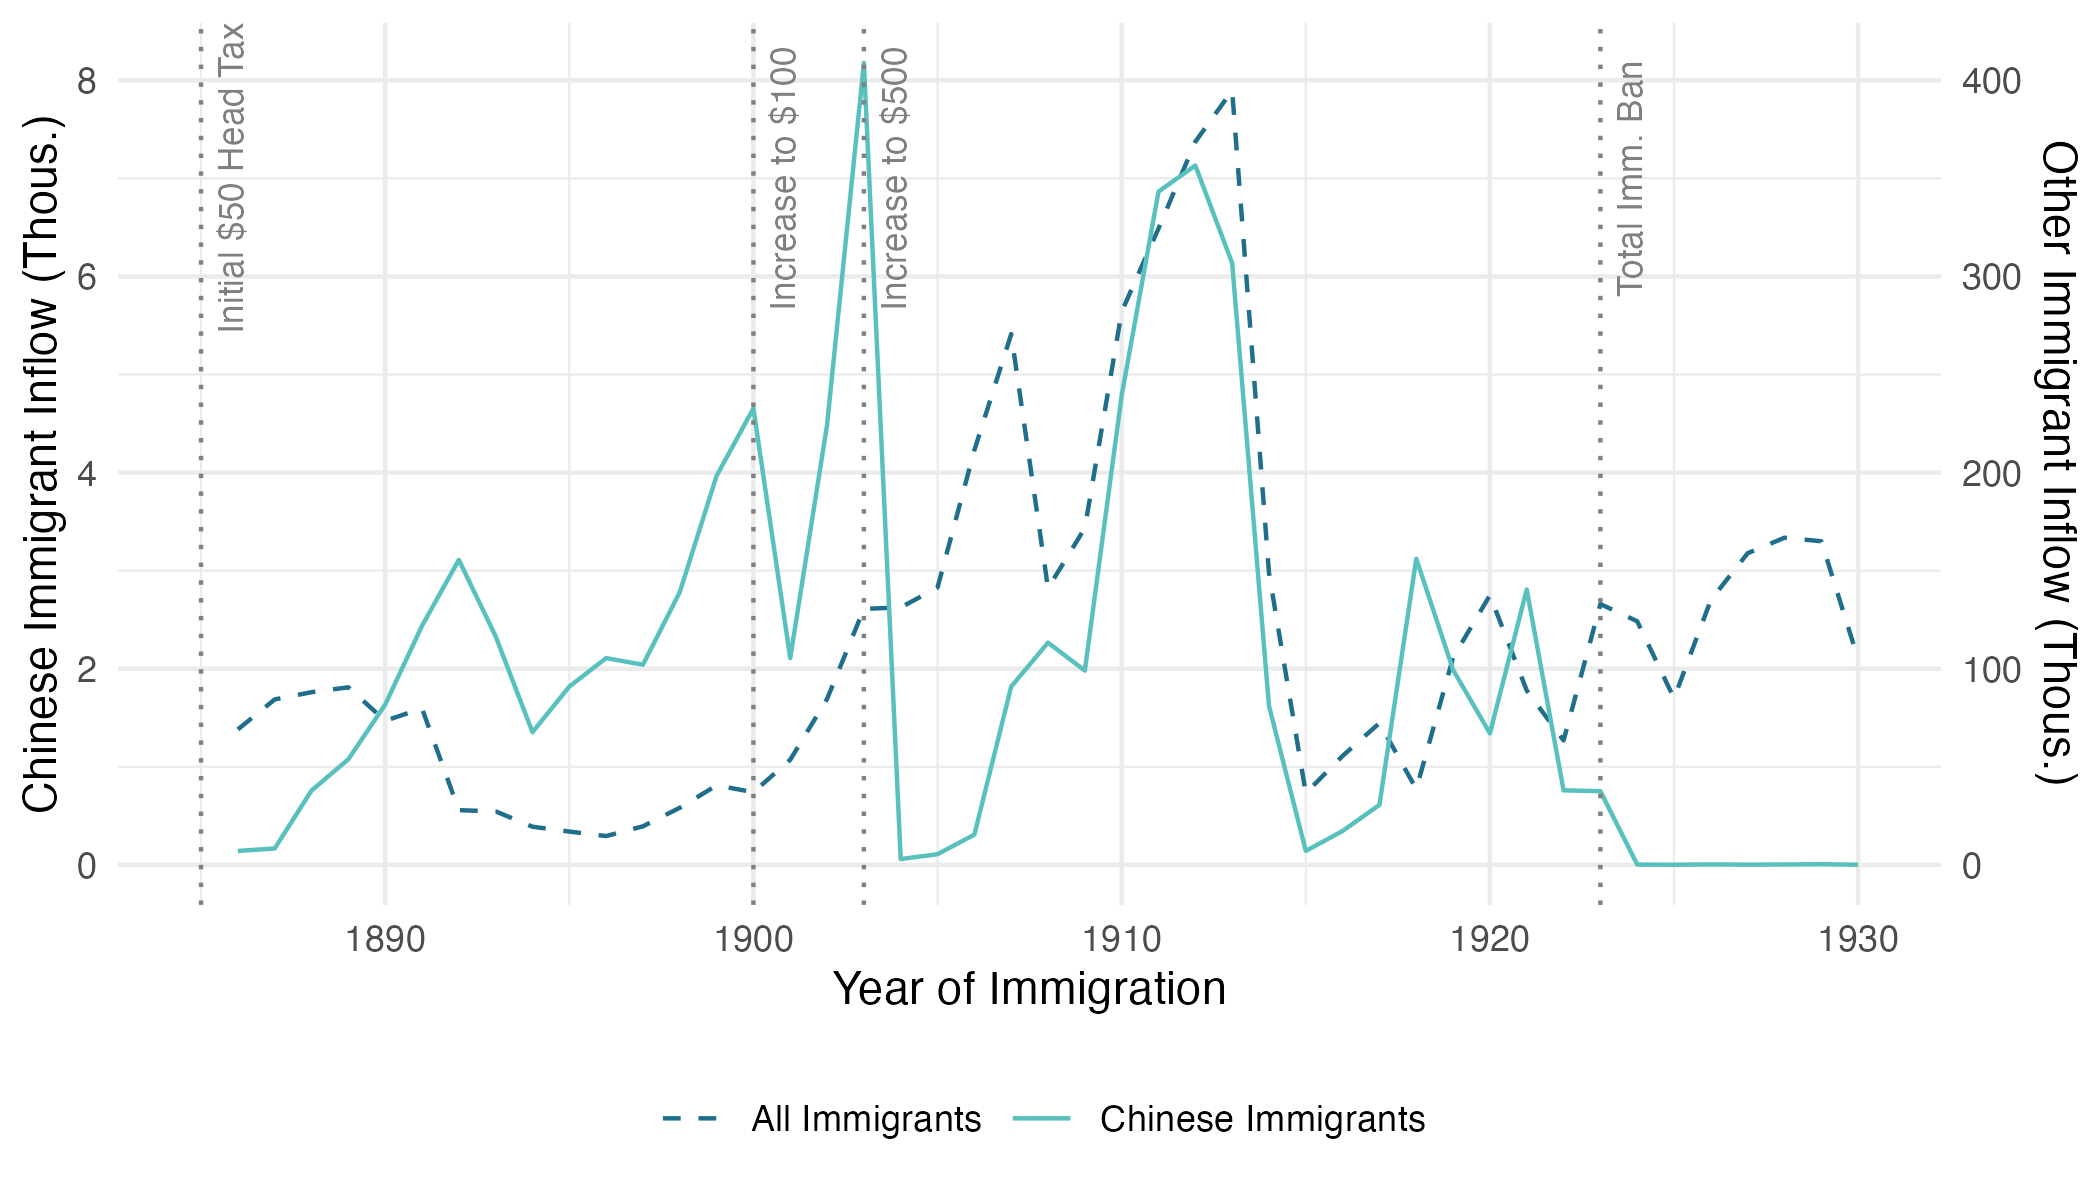
\includegraphics[width=\textwidth]{../../figs/fig1_immflow.png}
    \label{fig:inflow}
\end{figure}

I begin by showing the flow of both Chinese immigrants and all immigrants into Canada between 1886 and 1930 in Figure \ref{fig:inflow}.\footnote{Because the Chinese Register was first created when the Chinese Head Tax was implemented partway through 1885, I exclude years prior to 1886, the first full year where all immigrants were recorded in the Register.}
Chinese immigration to Canada (indicated by the solid line) during this period peaked in 1903, with 8,177 new Chinese immigrants registered in that year alone. In the following year, after the head tax was increased from \$100 to \$500 on January 1st of 1904, only 59 new Chinese immigrants were registered. This pattern of a sharp drop in Chinese immigration following an increase in the Head Tax is also visible in 1901 (following an increase in the Head Tax from \$50 to \$100), and in 1886 (following the introduction of the Head Tax), and can not be explained by trends in overall immigration to Canada (indicated by the dashed line).

I test for the statistical significance of these drops using the following specification: 
\begin{multline}
    \label{eq:immflow1}
    FLOW_{China,t} = \alpha_0 + \alpha_1 HKEMIG_t + \alpha_2 CANIMMIG_t + \alpha_3 POPSTOCK_{China, t-1} \\ + \alpha_4 (POPSTOCK_{China, t-1})^2 + \sum_{\tau \in \mathcal{T}^d} \gamma_\tau \mathbbm{1}[TAX_t = \tau]
\end{multline}

The dependent variable, $FLOW_{China,t}$, represents the inflow of Chinese immigrants in year $t$ to Canada as recorded in the Chinese Register. To account for `push' factors, the regression includes $HKEMIG_t$, total emigration out of Hong Kong in each year as recorded in the Harbourmaster reports,\footnote{As discussed in Section 3.1.2, the majority of Chinese immigrants to Canada departed from Hong Kong. Additionally, since emigration to Canada comprised less than 8\% of total emigration from Hong Kong even at its peak, there were likely no spillover effects of Canadian immigration policy on total Hong Kong emigration.} and to account for `pull' factors the regression includes $CANIMMIG_t$, total immigration into Canada in each year.\footnote{Data on total annual immigration to Canada is obtained from a report by \citet{canimm}.}

While these controls account for factors influencing emigration from Southern China and immigration to Canada independently, they do not control for the Canada-specific push from Southern China, or the Southern China-specific pull from Canada. To this end, I include controls for $POPSTOCK_{China,t-1}$, the lagged stock of Chinese immigrants living in Canada, and $(POPSTOCK_{China,t-1})^2$, which \citet{Clarketal2007} show to be the largest determinants of migration flows outside of immigration policy.\footnote{I compute the stock of Chinese immigrants living in Canada every ten years starting in 1871 using the number of people born in China as reported in the Canadian Census. I then interpolate the population stock in intercensal years using a natural cubic spline. Results are robust to using linear interpolation.}

Finally, the last term flexibly captures the effect of the Head Tax. $d$ indexes the dataset, $\mathcal{T}^d$ represents the set of tax indicators that can be used given the data, and $TAX_t$ represents the Head Tax amount in year $t$. When I use Chinese Register data, $\mathcal{T}^{register} = \{\$100,\$500\}$, leaving the \$50 tax as the excluded group since complete inflow data was not recorded in the Register prior to 1886. The primary objects of interest are therefore $\gamma_{100}$ and $\gamma_{500}$, which represent the effects of the \$100 and \$500 Head Taxes respectively on Chinese immigration to Canada, relative to the \$50 Head Tax.

Column (1) of Table \ref{tab:immflow} presents the results of equation \eqref{eq:immflow1}. While the estimate of $\gamma_{100}$ is negative, it is only identified off of three years (1901-1903) and is not significantly negative at the 95\% level. The estimate of $\gamma_{500}$, on the other hand, is large and significantly negative at the 95\% confidence level, implying that the \$500 Head Tax was associated with 8,803 fewer Chinese immigrants per year relative to the \$50 Head Tax. This corresponds to a 79.6\% drop in immigration relative to a predicted annual immigration level of 11,051 between 1904 and 1923. 

To supplement this analysis, I also estimate equation \eqref{eq:immflow1} using Census data rather than Register data. Census data captures immigration prior to 1886, allowing me to include an indicator for the \$50 Head Tax such that $\mathcal{T}^{census} = \{\$50,\$100,\$500\}$ and to estimate the effect of each of the Head Tax amounts relative to no Head Tax. Column (4) of Table \ref{tab:immflow} presents these results. 
I find qualitatively similar results as when using the Register data -- effects in years with smaller quantities of the Head Tax are negative although not significant, while the estimate of $\gamma_{500}$ is large and significantly negative, corresponding to a 54.0\% drop in immigration\footnote{Note that the recorded number of immigrants in the Census is heavily attenuated relative to the Chinese Register because of outmigration between decennial censuses. 
To partially account for for the change in outmigration bias between years, I control for $CANIMMIG_t$ as recorded in the Census rather than by official immigration statistics. Although outmigration rates likely differ for Chinese immigrants and other immigrants, I consider this to be approximately accurate in accounting for Census-related biases, and the qualitative similarity between results in column (1) and column (4) lend support to the accuracy of these results.}

Note that the drops in immigration inflows observed in Figure \ref{fig:inflow} can be interpreted in two ways. If we think of Chinese immigration as growing rapidly over this time period (excluding World War I, when immigration overall very low), then we can interpret these drops as persistent decreases in the number of Chinese immigrants -- i.e. we conjecture that the peaks of Chinese immigration in 1903 and the early 1910s would have been even higher in the absence of the Chinese Head Tax. On the other hand, if we think of Chinese immigration as growing more slowly, and perhaps even beginning to decrease near the turn of the century, then we can interpret these drops as being only temporary -- i.e. that within just a couple years of a Head Tax increase, Chinese immigration bounced back completely to its original level.

My analysis in equation \eqref{eq:immflow1} only captures the effect of the head tax under the first framework. To test for temporary drops in immigration, I modify equation \eqref{eq:immflow1} to include the interaction between the Head Tax indicators and $2YR_t$, an indicator for whether $t$ is within two years of a change in the Head Tax. The resulting estimating equation is as follows: 

\begin{multline}
    \label{eq:immflow2}
    FLOW_{China,t} = \alpha_0 + \alpha_1 HKEMIG_t + \alpha_2 CANIMMIG_t + \alpha_3 POPSTOCK_{China, t-1} \\ + \alpha_4 (POPSTOCK_{China, t-1})^2 + \sum_{\tau \in \mathcal{T}^d} \gamma^{2YR}_\tau \mathbbm{1}[TAX_t = \tau]\times 2YR_t
\end{multline}

Estimation of equation \eqref{eq:immflow2} using Register data is presented in column (2) of Table \ref{tab:immflow}. While the results are again qualitatively similar to my first specification (no significant effect of the \$100 tax, and a significantly negative effect of the \$500 tax), the adjusted $R^2$ in column (2) is 0.3 compared to 0.75 in column (1), indicating that much less of the variation in immigration inflows is explained by only allowing the effect of the tax increases to last two years. Column (3) combines equations \eqref{eq:immflow1} and \eqref{eq:immflow2}, allowing for both persistent effects of the Head Tax increases (captured by $\gamma_{\tau}$) and temporary effects (captured by $\gamma_{\tau}^{2YR}$). 
Allowing for temporary effects does not appear to meaningfully change $\gamma_{500}$, although the sign of $\gamma_{100}$ flips, suggesting that most of the effect of the \$100 Head Tax on Chinese immigration is in the first two years (although the \$100 Head Tax was only in effect for three years in total).

I repeat this analysis using Census data in columns (5) and (6). Once again, adding the temporary effects to the equation does not appear to meaningfully change the persistent effects in the top three rows of column (6), although column (5) suggests that the temporary effects alone have significant explanatory power in the Census data, perhaps indicating that the effect of the Head Tax on return migration was more temporary.

\begin{table}[!h]
    \centering 
    \renewcommand{\arraystretch}{1.2}
    \resizebox{\textwidth}{!}{
    \begin{threeparttable}
        \caption{Summary of regression results showing the relationship between the Chinese Head Tax and Chinese immigrant inflow to Canada using equations \eqref{eq:immflow1} and \eqref{eq:immflow2}.}
        \label{tab:immflow}
        
% Table created by stargazer v.5.2.3 by Marek Hlavac, Social Policy Institute. E-mail: marek.hlavac at gmail.com
% Date and time: Wed, Apr 12, 2023 - 12:49:22
\begin{tabular}{@{\extracolsep{5pt}}lcccccccccc} 
\\[-1.8ex]\hline 
\hline \\[-1.8ex] 
 & \multicolumn{3}{c}{Chinese Register} & \multicolumn{7}{c}{Canadian Census} \\ 
\\[-1.8ex] & (1) & (2) & (3) & (4) & (5) & (6) & (7) & (8) & (9) & (10)\\ 
\hline \\[-1.8ex] 
 $TAX$ & 0.704 & $-$4.733$^{*}$ &  & 2.432$^{***}$ & 1.080 &  & $-$2.508$^{***}$ &  & $-$0.692 &  \\ 
  & (1.339) & (2.617) &  & (0.386) & (0.890) &  & (0.890) &  & (0.524) &  \\ 
  & & & & & & & & & & \\ 
 \$50 Tax &  &  & $-$2,251.000 &  &  & 204.100 &  & $-$469.400 &  & $-$28.670 \\ 
  &  &  & (1,485.000) &  &  & (317.000) &  & (394.200) &  & (183.700) \\ 
  & & & & & & & & & & \\ 
 \$100 Tax &  &  & $-$1,283.000 &  &  & 931.900$^{*}$ &  & $-$584.900 &  & $-$395.200 \\ 
  &  &  & (2,292.000) &  &  & (513.500) &  & (597.600) &  & (312.000) \\ 
  & & & & & & & & & & \\ 
 \$500 Tax &  &  & $-$4,336.000$^{*}$ &  &  & 973.900 &  & $-$1,592.000$^{**}$ &  & $-$535.800 \\ 
  &  &  & (2,406.000) &  &  & (591.100) &  & (661.300) &  & (403.200) \\ 
  & & & & & & & & & & \\ 
Time Trends & No & Yes & Yes & No & Yes & Yes & Yes & Yes & Yes & Yes \\ 
Ctrl. for Total Immigration & No & No & No & No & No & No & Yes & Yes & Yes & Yes \\ 
\hline \\[-1.8ex] 
Observations & 44 & 44 & 44 & 54 & 54 & 54 & 41 & 41 & 41 & 41 \\ 
Adjusted R$^{2}$ & $-$0.017 & 0.213 & 0.250 & 0.422 & 0.506 & 0.518 & 0.692 & 0.682 & 0.373 & 0.381 \\ 
\hline \\[-1.8ex] 
\end{tabular} 

        \begin{tablenotes}
            \item $^{*}$p$<$0.1; $^{**}$p$<$0.05; $^{***}$p$<$0.01
            \item 
            \item \textbf{Notes:} The outcome variable $FLOW_{China,t}$ is measured using Chinese Register data in columns (1)-(3), which are exact records of legal Chinese immigrants to Canada betwen 1886 and 1923, and using Canadian Census data in columns (4)-(6) \citep{chineseregister,census1901,census1911,census1921}. Note that Year of Immigration was only asked as a census question beginning in 1901 and so I only use the 1901, 1911, and 1921 censuses -- to minimize bias from outmigration while still capturing immigration before the Head Tax, I restrict this sample to span from 1880-1920. 
            All regressions include controls for $HKEMIG_t$ (total emigration from Hong Kong in year $t$ as obtained from annual Hong Kong Harbormaster Reports), $CANIMMIG_t$ (total immigration to Canada in year $t$ as obtained from [source] for columns (1)-(3) and the Canadian census for columns (4)-(6)), $POPSTOCK_{China, t-1}$ (lagged population stock of Chinese immigrants in Canada as interpolated from Canadian census data using a natural cubic spline), and $(POPSTOCK_{China, t-1})^2$, as well as a constant.
        \end{tablenotes}
    \end{threeparttable}
    }
\end{table}

Finally, as a placebo test, I estimate the effects of the Head Tax on immigration inflows for countries other than China, and present the results in Appendix C. My results indicate that the effects of the Head Tax on Chinese immigration as observed in Figure \ref{fig:inflow} and in the regression results in Table \ref{tab:immflow} are not spurious or related to broader Canadian immigration policy at the time, and also suggests that the Head Tax did not have significant spillover effects on other immigrant groups. 